\chapter{Implementation}
\label{chap:Implementation}

\section{Technical Setup}

The implementation leverages SAP's Business Technology Platform (BTP) and Joule platform to create an AI-powered agent system for addressing missing component issues in production orders. The technical architecture follows a microservices approach with the following key components:

\subsection{Technology Stack}

\begin{table}[h]
\centering
\begin{tabular}{@{}ll@{}}
\toprule
\textbf{Component} & \textbf{Technology} \\
\midrule
AI Platform & SAP Joule \\
Backend System & SAP S/4HANA Manufacturing Public Cloud \\
AI Model & OpenAI GPT-4o \\
Deployment Platform & SAP Business Technology Platform (BTP) \\
User Interface & SAP UI5 Integration Cards \\
CI/CD Pipeline & Jenkins with Joule-specific libraries \\
\bottomrule
\end{tabular}
\caption{Technology Stack Overview}
\end{table}


\section{Development Steps}

\subsection{Core Functions Implementation}

The implementation consists of several core functions that handle different aspects of the production order analysis:

\subsubsection{Production Order Management}
\begin{itemize}
    \item \texttt{get\_production\_order\_object.yaml}: Retrieves comprehensive production order details
    \item \texttt{get\_po\_components.yaml}: Extracts component list for analysis
    \item \texttt{get\_single\_status\_prod\_order.yml}: Provides order status information
\end{itemize}

\subsubsection{Component Analysis}
\begin{itemize}
    \item \texttt{get\_bom.yaml}: Retrieves Bill of Materials for materials
    \item \texttt{get\_ref\_orders.yaml}: Finds reference production orders with similar materials
    \item \texttt{execute\_atp\_check.yaml}: Performs Available-to-Promise validation
\end{itemize}

\subsubsection{AI-Powered Alternative Discovery}
\begin{itemize}
    \item \texttt{find\_alternative\_agent\_call.yaml}: Main AI orchestration function
    \item Implements intelligent component matching algorithms
    \item Provides conversational interface for user interaction
\end{itemize}

\subsection{AI Agent Configuration}

The AI agent is configured with specialized instructions for manufacturing component analysis:

\begin{verbatim}
expertIn: "You are expert to give alternative suggestions for a missing component of a production order"
initialInstructions: |
  Goal: Find possible alternative components that might replace a missing component 
  of the target production order by reviewing other production orders that use similar components.
  
  1. Initial Verification
  a. Verify that the target production order has at least one missing component.
  b. If there is more than one missing component, identify which specific component 
     you need to find an alternative for.
  
  2. Get Target Order's Components
  a. Use the get_po_components tool to retrieve the complete list of components.
  b. Capture both Material Name and BOM (BillOfMaterialItemNumber).
  
  3. Find Potential Alternative Components
  a. Get reference production orders using get_ref_orders tool.
  b. Compare component lists with 50%+ matching criteria.
  c. Identify functionally similar components as alternatives.
  
  4. Final Output to User
  a. Display alternatives in markdown table format.
  b. Include Material Name and Production Order ID.
\end{verbatim}

\subsection{Data Flow Process}

The implementation follows a structured workflow as illustrated in Figure~\ref{fig:implementation-flow} and Figure~\ref{fig:data-flow}:

\begin{figure}[h]
    \centering
    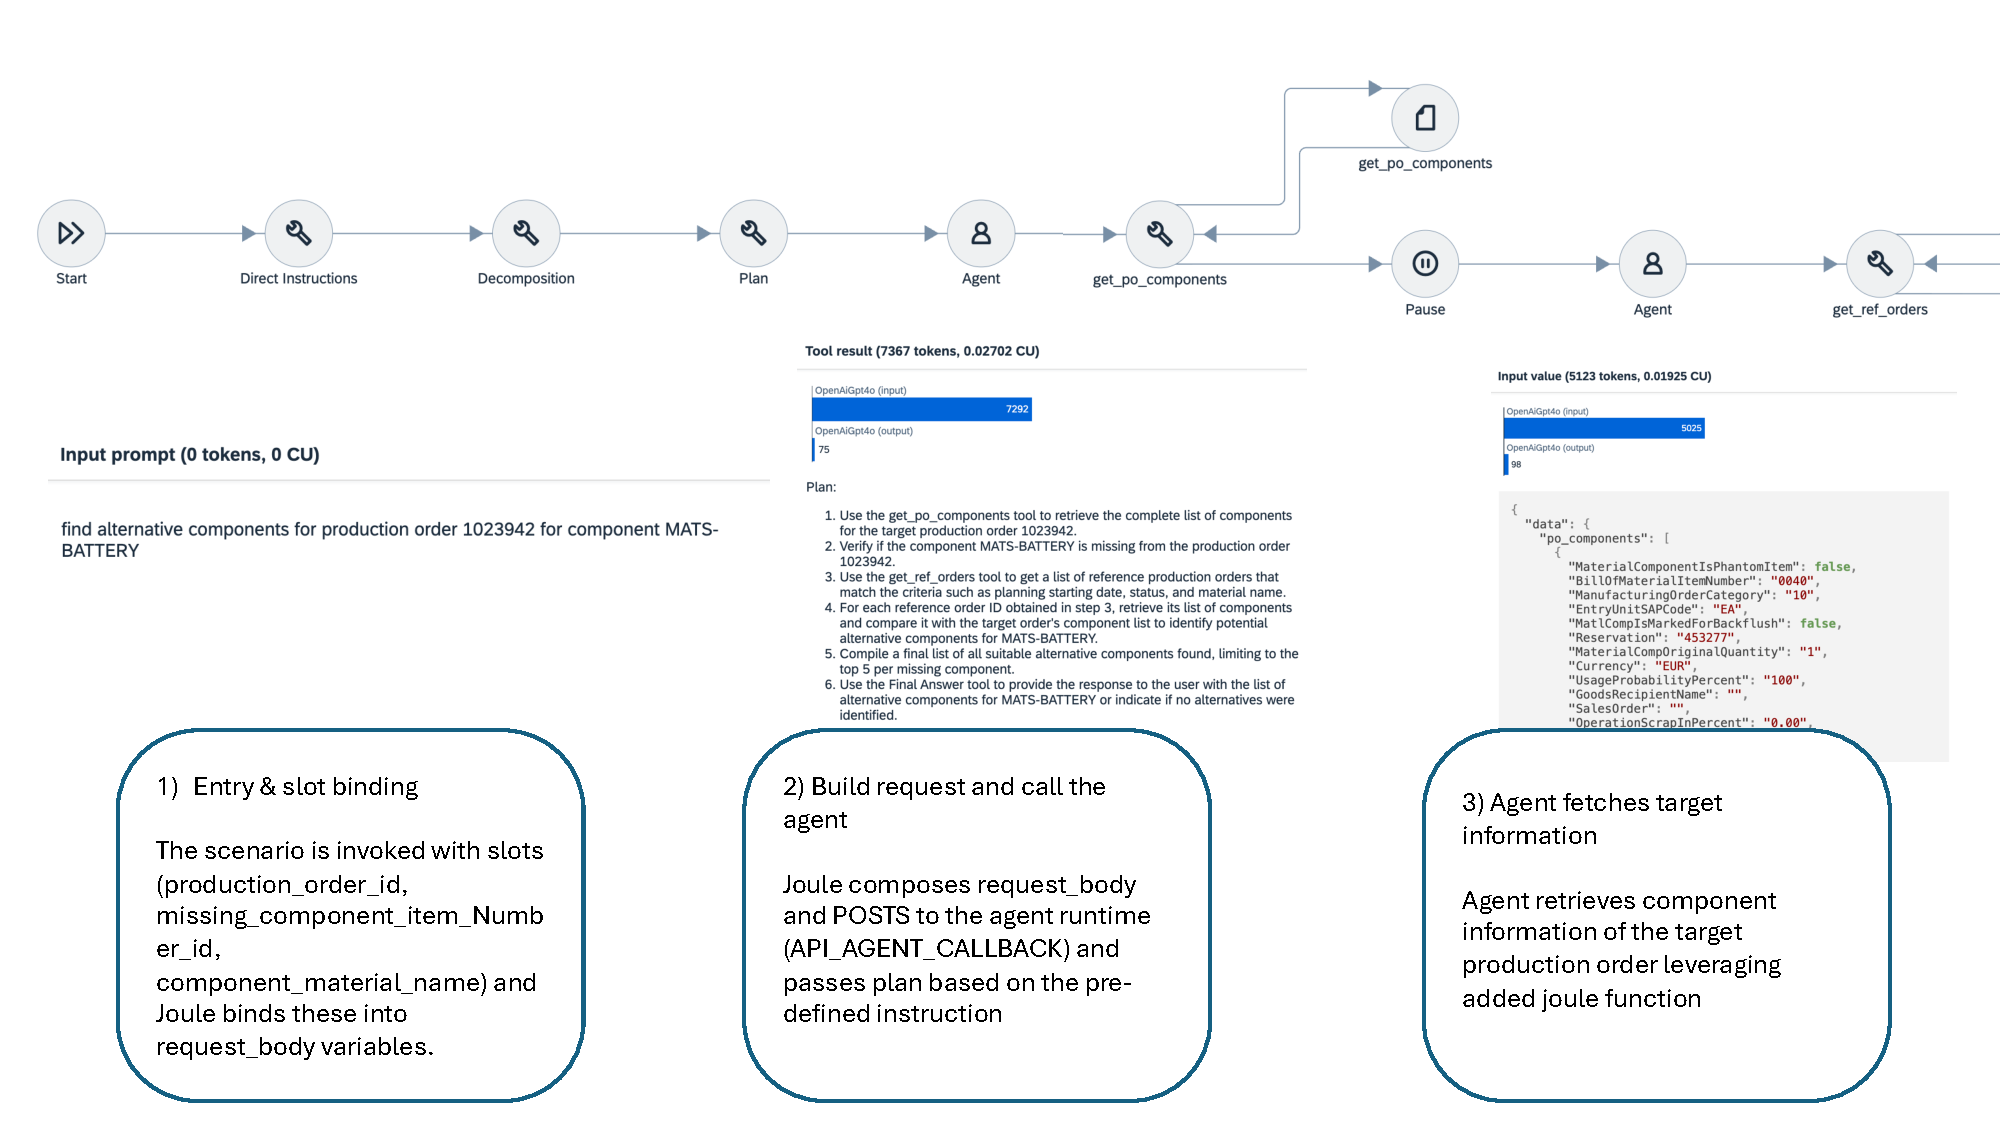
\includegraphics[width=1.0\textwidth]{graphic/flow-1.pdf}
    \caption{Implementation Flow Diagram for Production Order Release Agent}
    \label{fig:implementation-flow}
    \end{figure}
    
    \begin{figure}[h]
        \centering
        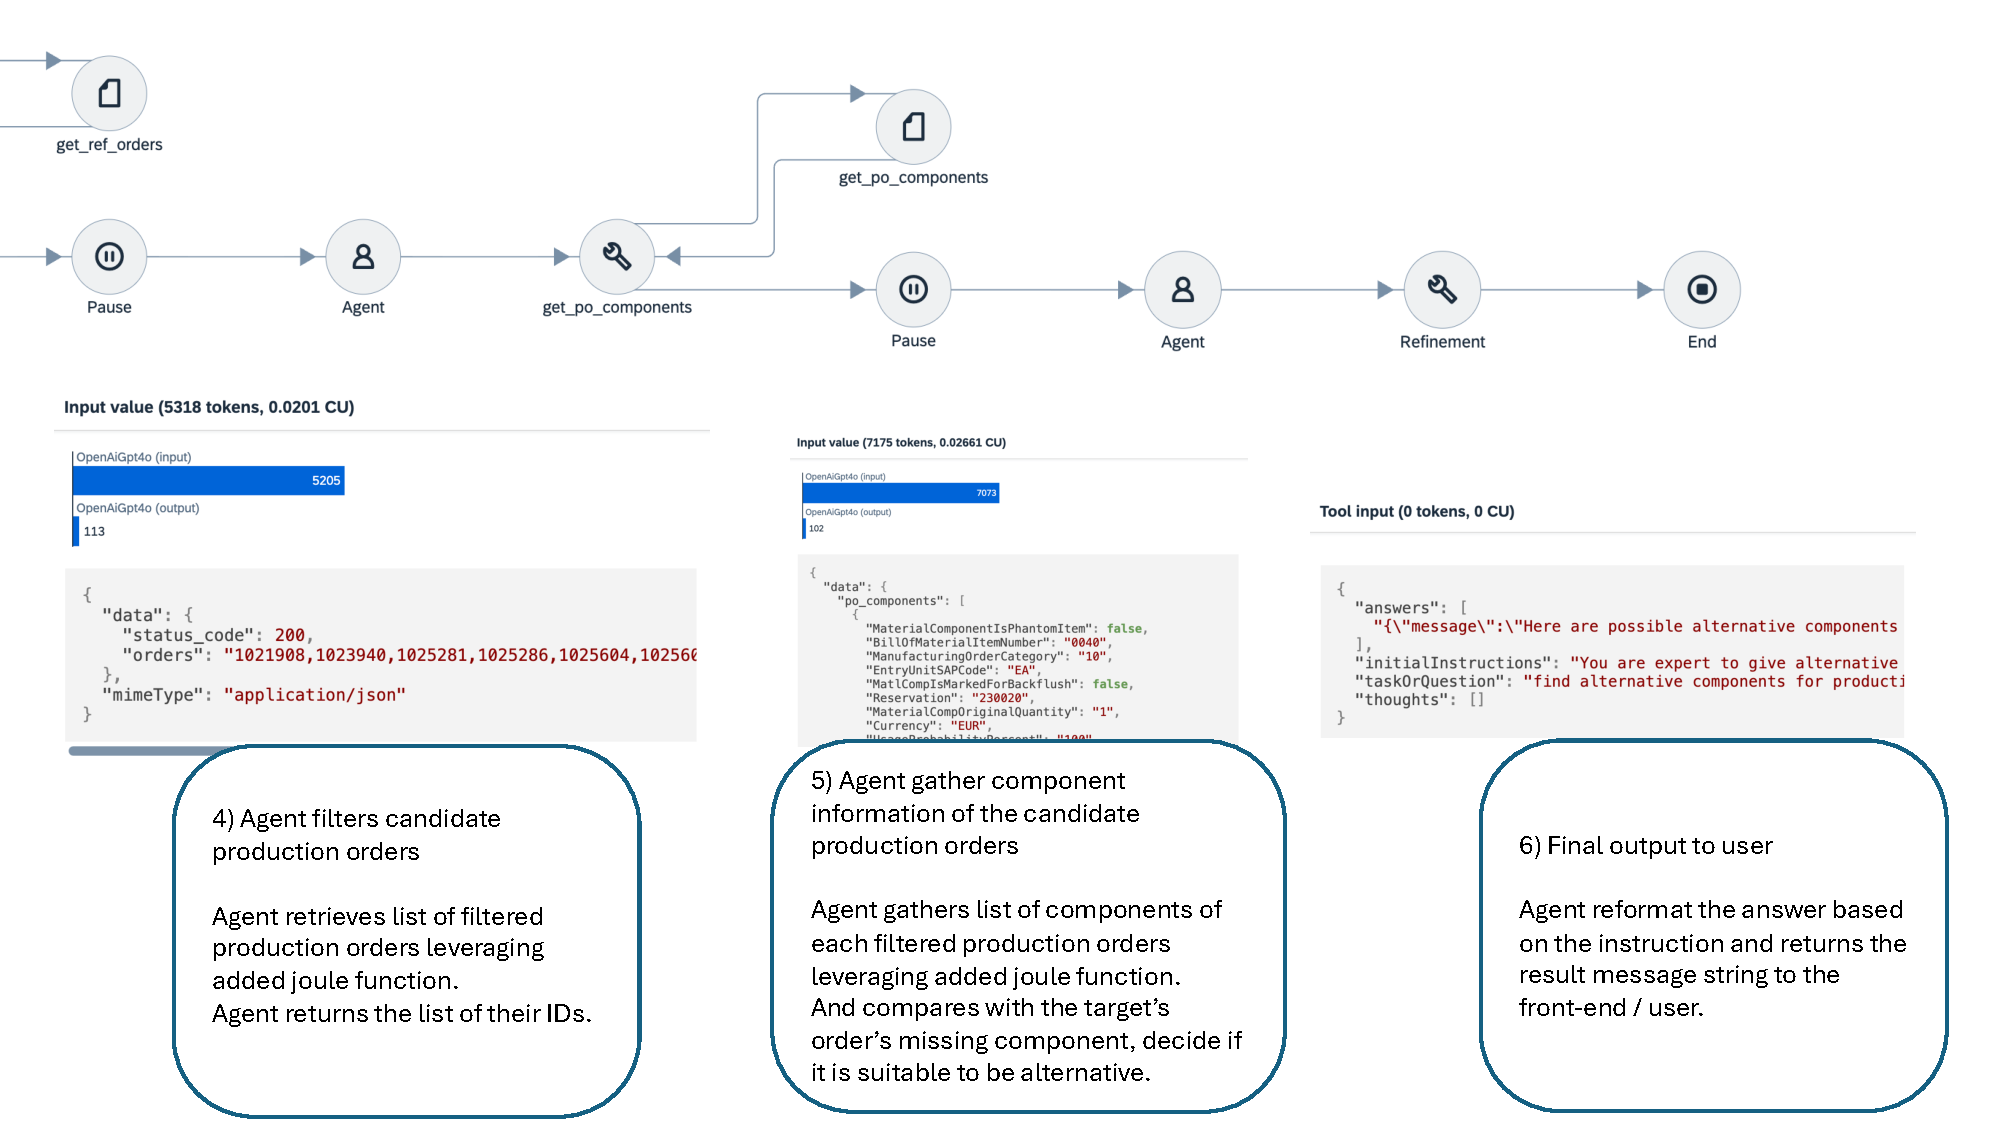
\includegraphics[width=1.0\textwidth]{graphic/flow-2.pdf}
        \caption{Data Flow Process Diagram for Production Order Release Agent}
        \label{fig:data-flow}
    \end{figure}

\section{UI Mockups and UX}

\subsection{User Experience Design}

The system provides an intuitive conversational interface with the following key features:

\begin{itemize}
    \item \textbf{Conversational Interface}: Natural language interaction with the AI agent
    \item \textbf{Rich UI Components}: SAP UI5 integration cards for enhanced visualization
    \item \textbf{Interactive Decision Support}: Quick reply buttons for user responses
    \item \textbf{Multi-language Support}: 50+ language internationalization
\end{itemize}

\subsection{Key Features}

\subsubsection{Intelligent Component Matching}
\begin{itemize}
    \item \textbf{Similarity Analysis}: 50\%+ component list matching criteria
    \item \textbf{Functional Equivalence}: AI determines functional similarity of components
    \item \textbf{Historical Validation}: Only suggests alternatives from successfully completed orders
    \item \textbf{Status Filtering}: Considers only released, confirmed, or completed orders
\end{itemize}

\subsubsection{Integration Capabilities}
\begin{itemize}
    \item \textbf{SAP S/4HANA Integration}: Direct API calls to manufacturing systems
    \item \textbf{Process Automation}: Integration with SAP PAB for workflow automation
    \item \textbf{Real-time Data}: Live data from production order management
    \item \textbf{ATP Integration}: Real-time availability checking
\end{itemize}
